Une exposition d'art contemporain a lieu dans une salle en forme de pavé droit de largeur 6 m, de longueur 8 m et de hauteur 4 m. 

Elle est représentée par le parallélépipède rectangle $OBCDEFGH$ où $OB = 6$ m, $OD = 8$ m et $OE = 4$ m.

On utilise le repère orthonormé $\Rijk$ tel que $\vect{\imath} = \dfrac16\vect{\text{OB}}, \vect{\jmath} = \dfrac18\vect{\text{OD}}$ et $\vect{k} =\dfrac18\vect{\text{OE}}$.

\begin{center}
	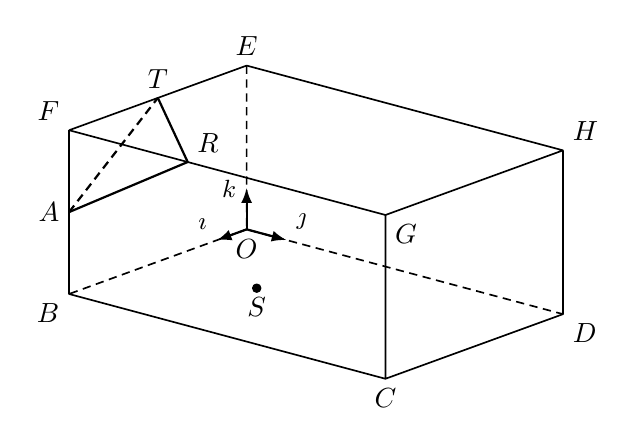
\begin{tikzpicture}[x={(-160:0.4cm)},y={(-15:0.52cm)},z={(90:0.52cm)},line join=bevel]
		\coordinate (O) at (0,0,0) ; \draw (O) node[below] {$O$} ;
		\coordinate (B) at (6,0,0) ; \draw (B) node[below left] {$B$} ;
		\coordinate (D) at (0,8,0) ; \draw (D) node[below right] {$D$} ;
		\coordinate (C) at (6,8,0) ; \draw (C) node[below] {$C$} ;
		\coordinate (E) at (0,0,4) ; \draw (E) node[above] {$E$} ;
		\coordinate (F) at (6,0,4) ; \draw (F) node[above left] {$F$} ;
		\coordinate (H) at (0,8,4) ; \draw (H) node[above right] {$H$} ;
		\coordinate (G) at (6,8,4) ; \draw (G) node[below right] {$G$} ;
		\draw[thick,->,>=latex] (O)--++(1,0,0) node[above left=0pt,font=\small] {$\vect{\imath}$} ;
		\draw[thick,->,>=latex] (O)--++(0,1,0) node[above right=0pt,font=\small] {$\vect{\jmath}$} ;
		\draw[thick,->,>=latex] (O)--++(0,0,1) node[left=0pt,font=\small] {$\vect{k}$} ;
		\draw[semithick,densely dashed] (O)--(B) (E)--(O)--(D) ;
		\draw[semithick] (B)--(F)--(G)--(C)--cycle (F)--(E)--(H)--(G)--cycle (C)--(D)--(H) ;
		%autres points et tracés
		\coordinate (A) at (6,0,2) ; \draw (A) node[left] {$A$} ;
		\coordinate (R) at (6,3,4) ; \draw (R) node[above right] {$R$} ;
		\coordinate (T) at (3,0,4) ; \draw (T) node[above] {$T$} ;
		\coordinate (S) at (3,2.5,0) ; \filldraw (S) circle[radius=1.5pt] node[below] {$S$} ;
		\draw[thick] (A)--(R)--(T) ; \draw[thick,densely dashed] (A)--(T) ;
	\end{tikzpicture}
\end{center}

Dans ce repère on a, en particulier $C(6;8;0)$, $F(6;0;4)$ et $G(6;8;4)$.

Une des œuvres exposées est un triangle de verre représenté par le triangle $ART$ qui a pour sommets $A(6;0;2)$, $R(6;3;4)$ et $T(3;0;4)$, Enfin, $S$ est le point de coordonnées $\left(3;\dfrac52;0\right)$.

\begin{enumerate}
	\item 
	\begin{enumerate}
		\item Vérifier que le triangle $ART$ est isocèle en $A$.
		\item Calculer le produit scalaire $\vect{\text{AR}} \cdot \vect{\text{AT}}$.
		\item En déduire une valeur approchée à $0,1$ degré près de l'angle $\widehat{\text{RAT}}$.
	\end{enumerate}
	\item 
	\begin{enumerate}
		\item Justifier que le vecteur $\vect{n}\begin{pmatrix}2\\-2\\3\end{pmatrix}$ est un vecteur normal au plan $(ART)$.
		\item En déduire une équation cartésienne du plan $(ART)$.
	\end{enumerate}
	\item Un rayon laser dirigé vers le triangle $ART$ est émis du plancher à partir du point $S$. On admet que ce rayon est orthogonal au plan $(ART)$.
	\begin{enumerate}
		\item Soit $\Delta$ la droite orthogonale au plan $(ART)$ et passant par le point $S$.
		
		Justifier que le système ci-dessous est une représentation paramétrique de la droite $\Delta$ : \[ \begin{dcases} x=3+2k \\ y=\frac52 -2k \quad \text{, avec} k \in \R \\ z=\phantom{2+}3k \end{dcases} \]
		\item Soit $L$ le point d'intersection de la droite $\Delta$, avec le plan $(ART)$.
		
		Démontrer que $L$ a pour coordonnées $\left(5;\dfrac12;3\right)$.
	\end{enumerate}
	\item L'artiste installe un rail représenté  par le segment $[DK]$ où $K$ est le milieu du segment $[EH]$.
	
	Sur ce rail, il positionne une source lumineuse laser en un point $N$ du segment $[DK]$ et il oriente ce second rayon laser vers le point $S$.
	
	\begin{center}
		\begin{tikzpicture}[x={(-160:0.4cm)},y={(-15:0.52cm)},z={(90:0.52cm)},line join=bevel]
			\coordinate (O) at (0,0,0) ; \draw (O) node[below] {$O$} ;
			\coordinate (B) at (6,0,0) ; \draw (B) node[below left] {$B$} ;
			\coordinate (D) at (0,8,0) ; \draw (D) node[below right] {$D$} ;
			\coordinate (C) at (6,8,0) ; \draw (C) node[below] {$C$} ;
			\coordinate (E) at (0,0,4) ; \draw (E) node[above] {$E$} ;
			\coordinate (F) at (6,0,4) ; \draw (F) node[above left] {$F$} ;
			\coordinate (H) at (0,8,4) ; \draw (H) node[above right] {$H$} ;
			\coordinate (G) at (6,8,4) ; \draw (G) node[below right] {$G$} ;
			\draw[thick,->,>=latex] (O)--++(1,0,0) node[above left=0pt,font=\small] {$\vect{\imath}$} ;
			\draw[thick,->,>=latex] (O)--++(0,1,0) node[above right=0pt,font=\small] {$\vect{\jmath}$} ;
			\draw[thick,->,>=latex] (O)--++(0,0,1) node[left=0pt,font=\small] {$\vect{k}$} ;
			\draw[semithick,densely dashed] (O)--(B) (E)--(O)--(D) ;
			\draw[semithick] (B)--(F)--(G)--(C)--cycle (F)--(E)--(H)--(G)--cycle (C)--(D)--(H) ;
			%autres points et tracés
			\coordinate (A) at (6,0,2) ; \draw (A) node[left] {$A$} ;
			\coordinate (R) at (6,3,4) ; \draw (R) node[above right] {$R$} ;
			\coordinate (T) at (3,0,4) ; \draw (T) node[above] {$T$} ;
			\coordinate (S) at (3,2.5,0) ;
			\draw[thick] (A)--(R)--(T) ; \draw[thick,densely dashed] (A)--(T) ;
			\coordinate (L) at (5,0.5,3) ;
			\coordinate (K) at ($(E)!0.5!(H)$) ; \draw (K) node[above] {$K$} ;
			\draw[semithick,densely dashed] (K)--(D) ;
			\coordinate (N) at (0,{23/5},{17/5}) ; 
			\draw[thick,red] (L)--(S)--(N) ;
			%point labélisés
			\filldraw (N) circle[radius=1.5pt] node[right] {$N$} ;
			\filldraw (L) circle[radius=1.5pt] node[below] {$L$} ;
			\filldraw (S) circle[radius=1.5pt] node[below] {$S$} ;
		\end{tikzpicture}
	\end{center}
	\begin{enumerate}
		\item Montrer que, pour tout réel $t$ de l'intervalle $[0;1]$, le point $N$ de coordonnées $(0;8 - 4t;4t)$ est un point du segment $[DK]$.
		\item Calculer les coordonnées exactes du point $N$ tel que les deux rayons laser représentés par les segments $[SL]$ et $[SN]$ soient perpendiculaires.
	\end{enumerate}
\end{enumerate}

